\PassOptionsToPackage{table}{xcolor}
\documentclass[times, 10pt]{thesisMDH}
\usepackage[useregional]{datetime2}
% Fonts: scalable Type 1 fonts (the class alone falls back to bitmap Computer Modern)
\usepackage{mathpazo}                 % Palatino-style math
\usepackage{tgpagella}                % TeX Gyre Pagella for body text
\usepackage[scale=0.92]{tgheros}      % TeX Gyre Heros for sans-serif
\usepackage{tgcursor}                 % TeX Gyre Cursor for monospace
\linespread{1.06}
\usepackage{float}
\usepackage{enumitem}
\usepackage{booktabs}
\usepackage{tabularx}
\usepackage{ragged2e}
\usepackage{etoolbox}
\newcolumntype{Y}{>{\RaggedRight\arraybackslash}X}   % wrapped, left-aligned
\newcolumntype{R}{>{\raggedleft\arraybackslash}X}    % wrapped, right-aligned
\usepackage{colortbl}
\usepackage{caption}
\definecolor{rowtint}{RGB}{237, 242, 250}
\captionsetup[table]{position=above, skip=6pt, font=small, labelfont={bf,color=primaryblue}}
\captionsetup[figure]{skip=6pt, font=small, labelfont={bf,color=primaryblue}}
\newcommand{\hd}[1]{\textcolor{white}{\textbf{#1}}}   % header cell
\renewcommand{\arraystretch}{1.3}
\AtBeginEnvironment{tabularx}{\small}
\AtBeginEnvironment{tabular}{\small}
\usepackage{siunitx}
\usepackage{parskip}
\usepackage{array}
\usepackage{xcolor}
\usepackage{titlesec}
\usepackage{fancyhdr}
\usepackage{mathtools}
\usepackage{amsmath, amssymb}
\usepackage{graphicx}
\usepackage[pdfborder={0 0 0},colorlinks=true,urlcolor=blue,citecolor=red,bookmarks=false]{hyperref}

% Colors
\definecolor{primaryblue}{RGB}{30, 80, 162}
\definecolor{lightgray}{RGB}{245, 245, 245}
\definecolor{tpgreen}{RGB}{0, 128, 0}
\definecolor{fpred}{RGB}{200, 0, 0}
\definecolor{fnred}{RGB}{200, 0, 0}
\definecolor{tnblue}{RGB}{0, 0, 180}

% Section formatting
\titleformat{\section}{\large\bfseries\color{primaryblue}}{\thesection}{0.6em}{}[\titlerule]
\titleformat{\subsection}{\normalsize\bfseries\color{primaryblue}}{\thesubsection}{0.6em}{}

\pagestyle{fancy}
\fancyhf{}
\rhead{\textcolor{gray}{\small ECG Heartbeat Classification for MAX78002}}
\lhead{\textcolor{gray}{\small D7043E, Data Mining -- Group 16}}
\rfoot{\thepage}

% Useful macros
\newcommand{\mat}[1]{\mathbf{#1}}
\newcommand{\T}{\top}
\newcommand{\tbd}[1][value]{\textcolor{fpred}{[#1]}}   % marks numbers to be filled from results/
\graphicspath{{figures/}{images/}}

\addbibresource{references.bib}

% Template originally by henrik.falk@mdh.se; adapted for the D7043E ECG project, Group 16

\fancyHeader{ECG Heartbeat Classification for MAX78002}{Ekpenyong, Sreenidhi, Sowmya}

\university{Luleå Technical University}

\department{School of Computer Science, Electrical and Space Engineering\\
Luleå, Sweden}

\subject{\textbf{Project Report\\ Group 16}\\ D7043E, Data Mining}
\thesisTitle{ECG Heartbeat Classification for Edge AI on the MAX78002}

\authorOne{Ekpenyong Esu Ekpenyong}{ekpekp-5@student.ltu.se}
\authorTwo{Sreenidhi Thallam}{sretha-5@student.ltu.se}
\authorThree{Sowmya Nelakurthi}{sownel-4@student.ltu.se}

\examiner{Rajkumar Saini}{LTU, Luleå}
%\supervisors{Supervisor\_Name (if any)\textsuperscript{1}}{University, location}
%\companySupervisors{Supervisor\_Name (if any)\textsuperscript{1}}{Company name, location}

\theDate{\today}

\begin{document}
\titlePage
\tableofcontents
\newpage

\mainmatter
% ===== Submission 1: CRISP-DM stages 1-3 =====
\section{Business/Application Understanding}

\subsection{Application Scenario}

An electrocardiogram (ECG) records the electrical activity of the heart, and a cardiologist can tell from the shape and timing of each beat whether it is normal or originates from the wrong part of the heart. A day of continuous ECG contains around 100\,000 beats, so manual review of long recordings is impractical. Long-term monitoring depends on software that flags abnormal beats for the clinician to review.

This project builds the first stage of such a system: a small neural network that classifies one heartbeat as normal, supraventricular ectopic, ventricular ectopic or fusion. Ectopic beats originate outside the sinus node. Supraventricular ectopic beats start above the ventricles and are often close to normal in shape. Ventricular ectopic beats start in the ventricles and typically have a wide, abnormal QRS complex. A fusion beat occurs when a normal and a ventricular activation coincide.

Automatic beat classification is used in Holter recorders, hospital telemetry, wearable patches and smartwatches, and in screening where cardiologists are scarce. The target here is the wearable case, where running the classifier on the device has clear advantages over sending the signal to a server. The ECG stays on the device, which protects privacy. No network connection is needed. The result is available within milliseconds, which allows the device to alert the wearer. Transmitting raw ECG over a radio link also consumes far more energy than running a small model locally.

Potential users are patients wearing a monitor at home, clinicians reviewing flagged beats, device manufacturers, and researchers studying how such models generalise across people. This is a course project. The model is not a medical device and no clinical validation is claimed.

\subsection{Data Mining Objective}

\begin{description}
  \item[Input:] A fixed-length window of 256 samples (about 0.7 seconds at 360\,Hz) from a single ECG lead (MLII), cut around one annotated R-peak, filtered and normalised. The window covers 90 samples before the peak and 166 samples after it, so the model sees the P wave, the QRS complex and the T wave of one beat.
  \item[Output:] One of four classes for that beat: N (normal-type), S (supraventricular ectopic), V (ventricular ectopic) or F (fusion).
  \item[Type of task:] Supervised multiclass classification with four classes and a strong class imbalance.
\end{description}

\subsection{Project Objectives}

\begin{enumerate}[nosep]
  \item Distinguish N, S, V and F beats from a single-lead ECG window.
  \item Generalise to people the model has never seen, using a record-independent split.
  \item Stay usable when the ECG contains realistic noise from movement and muscle activity.
  \item Keep the model small enough for an embedded device: well under 2\,MB of weights.
  \item Make the model run on the MAX78002 CNN accelerator, verified by the Analog Devices software toolchain.
\end{enumerate}

\subsection{Success Criteria}

Accuracy alone is not a meaningful target. Almost 90\,\% of beats are normal, so a model that always predicts N reaches 90\,\% accuracy and detects nothing. The project is judged on the criteria in Table~\ref{tab:success-criteria}, all measured once on the test set DS2.

\begin{table}[H]
  \centering
  \caption{Success criteria. All are measured once, on DS2, after the model is frozen.}
  \label{tab:success-criteria}
  \rowcolors{2}{white}{rowtint}
  \begin{tabularx}{\linewidth}{l Y Y}
        \rowcolor{primaryblue}
    \hd{Criterion} & \hd{Metric} & \hd{Target} \\
    Predictive performance     & Macro-averaged F1 over the four classes on DS2 & $\geq 0.70$ \\
    Minority class performance & Recall (sensitivity) for S and for F on DS2     & $\geq 0.50$ each; V recall $\geq 0.85$ \\
    Noise robustness           & Drop in macro-F1 from clean ECG to 6\,dB SNR   & $\leq 0.15$ \\
    Model complexity           & Number of parameters and INT8 weight size      & $\leq 100\,000$ parameters; $\leq 200$\,kB \\
    MAX78002 compatibility     & ai8x quantisation and synthesis complete and produce C code & PASS on all four toolchain checks \\
    \bottomrule
  \end{tabularx}

\end{table}

In addition, the INT8 model must lose no more than 0.03 macro-F1 relative to the FP32 model, since only the INT8 model can be deployed.

\subsection{Constraints}

\textbf{Limited memory.} The MAX78002 accelerator has about 2\,MB of weight memory and a few hundred kilobytes for activations. Architectures common on GPUs do not fit.

\textbf{Fixed-point arithmetic.} The accelerator computes with 8-bit integers. Weights and activations must be quantised, and the model has to survive that with little loss.

\textbf{Class imbalance.} About nine in ten beats are normal and fusion beats are below 1\,\% of the data. A model can ignore the rare classes and still score well on accuracy.

\textbf{Few subjects.} The database has 48 records from 47 people. After removing the four paced records, I train on 22 records (DS1) and test on 22 others (DS2). This is a demanding generalisation task, and the rare classes are concentrated in a few records.

\textbf{Noise.} Real wearable ECG contains baseline drift, muscle activity and electrode movement. The training data is comparatively clean hospital ECG.

\textbf{Computational resources.} Training runs on a laptop or a modest GPU, which limits the size of hyperparameter searches.

\textbf{No physical board.} No MAX78002 development kit is available. Deployment is verified in software only, and no measured latency, power or on-device accuracy is reported.

\subsection{Risks and Challenges}

\begin{table}[H]
  \centering
  \caption{Main project risks and how they are handled.}
  \label{tab:risks}
  \rowcolors{2}{white}{rowtint}
  \begin{tabularx}{\linewidth}{Y Y Y}
        \rowcolor{primaryblue}
    \hd{Risk} & \hd{Why is it important?} & \hd{Proposed mitigation} \\
    The model cannot be synthesised for the MAX78002 &
    A model that does not run on the chip fails the main objective regardless of its accuracy. Discovering this late leaves no time to change the architecture. &
    Run a tiny model through the whole ai8x toolchain before tuning accuracy, and repeat after every architecture change. Use only convolution, pooling, ReLU and one small linear layer. \\
    \addlinespace
    Poor recall on S and F beats &
    S beats resemble normal beats and F beats are rare. Low recall on these classes makes the classifier of little clinical use. &
    Class-weighted loss and oversampling of S and F; monitor per-class recall during model selection; widen the input window if S recall stays low. \\
    \addlinespace
    Optimistic results from data leakage &
    Beats from the same person are highly similar. Any overlap between training and test inflates the score and hides the inter-patient gap. &
    Split strictly by record (DS1/DS2), validate by record inside DS1, and block test-set evaluation in code until the model is frozen. \\
    \addlinespace
    Large accuracy loss after INT8 quantisation &
    The deployed model is the INT8 one. If it is much worse than the FP32 model, the reported accuracy is not what the device delivers. &
    Scale inputs to the accelerator range, build with ai8x layers from the start, try post-training quantisation first, use quantisation-aware fine-tuning if needed. \\
    \addlinespace
    Model breaks down under noise &
    Wearable ECG is noisier than hospital ECG. A model that only works on clean signals is not useful in practice. &
    Baseline-wander removal, noise augmentation during training, and a dedicated noise test at 12, 6 and 0\,dB. \\
    \bottomrule
  \end{tabularx}

\end{table}

\section{Data Understanding}

\subsection{Dataset Description}

The main dataset is the MIT-BIH Arrhythmia Database from PhysioNet~\cite{moody2001mitbih}, the standard benchmark for beat classification, which allows comparison with published results.

\begin{table}[H]
  \centering
  \caption{Overview of the MIT-BIH Arrhythmia Database.}
  \label{tab:dataset}
  \rowcolors{2}{white}{rowtint}
  \begin{tabularx}{\linewidth}{l Y}
        \rowcolor{primaryblue}
    \hd{Property} & \hd{Value} \\
    Database           & MIT-BIH Arrhythmia Database, PhysioNet, version 1.0.0 \\
    Records            & 48 \\
    Subjects           & 47 (records 201 and 202 are from the same person) \\
    Channels           & 2 per record \\
    Sampling frequency & 360\,Hz \\
    Resolution         & 11 bits over a 10\,mV range \\
    Duration           & About 30 minutes per record, about 24 hours in total \\
    Annotations        & Beat-by-beat labels on the R-peak, made by two cardiologists with disagreements resolved \\
    Beat annotations   & About 110\,000 \\
    ECG leads          & First channel is modified limb lead II (MLII) in 46 records; second channel is usually V1, sometimes V2, V4 or V5. Records 102 and 104 have no MLII. \\
    \bottomrule
  \end{tabularx}

\end{table}

The recordings were made at Beth Israel Hospital in Boston between 1975 and 1979. Twenty-three records were selected at random from routine Holter tapes and twenty-five were selected because they contain rare but clinically important rhythms, which is why the database contains a usable number of abnormal beats despite its size.

For the noise experiment we use the MIT-BIH Noise Stress Test Database from the same source~\cite{moody1984noise}. It provides three half-hour recordings of pure noise, made with real electrodes on moving volunteers: baseline wander (\texttt{bw}), electrode motion artefact (\texttt{em}) and muscle artefact (\texttt{ma}). They are sampled at 360\,Hz, so they can be added directly to the arrhythmia recordings.

\subsection{Target Classes}

The database uses about fifteen beat symbols. They are grouped into the four required classes following the AAMI EC57 standard, which is also the grouping used in most inter-patient studies. Table~\ref{tab:classes} lists the mapping and the beat counts over the 44 records used.

\begin{table}[H]
  \centering
  \caption{Mapping from MIT-BIH beat symbols to the four target classes. Counts are produced by \texttt{prepare\_data.py} and stored in \texttt{results/split\_stats.csv}.}
  \label{tab:classes}
  \rowcolors{2}{white}{rowtint}
  \begin{tabularx}{\linewidth}{c l Y r}
        \rowcolor{primaryblue}
    \hd{Class} & \hd{MIT-BIH symbols} & \hd{Meaning} & \hd{Beats} \\
    N & \texttt{N}, \texttt{L}, \texttt{R}, \texttt{e}, \texttt{j} & Normal beat; left and right bundle branch block beats; atrial and nodal escape beats & 90\,125 \\
    S & \texttt{A}, \texttt{a}, \texttt{J}, \texttt{S}             & Atrial premature; aberrated atrial premature; nodal premature; supraventricular premature beats & 2\,781 \\
    V & \texttt{V}, \texttt{E}                                     & Premature ventricular contraction; ventricular escape beat & 7\,009 \\
    F & \texttt{F}                                                 & Fusion of ventricular and normal beat & 803 \\
    \bottomrule
  \end{tabularx}

\end{table}

\textbf{Excluded annotations.} Three kinds of labels are dropped. The preprocessing script counts every dropped beat, so the exclusions are reproducible.

\begin{itemize}[nosep]
  \item \textbf{Paced beats} (\texttt{/}) and \textbf{fusion of paced and normal beats} (\texttt{f}). These come from patients with pacemakers. The four paced records (102, 104, 107 and 217) are excluded entirely, as is standard practice, because the pacemaker spike is an artificial signal unrelated to the heart's own rhythm.
  \item \textbf{Unclassifiable beats} (\texttt{Q}). The annotators could not assign a class, so they cannot serve as training targets.
  \item \textbf{Non-beat annotations}, such as rhythm changes (\texttt{+}), noise markers (\texttt{\textasciitilde}) and signal-quality flags. These describe the recording, not a heartbeat, and are never counted as beats.
\end{itemize}

Excluding the paced records leaves 44 records, split evenly into DS1 and DS2 as described in Section~\ref{sec:record-selection}.

\subsection{Exploratory Data Analysis}

The full analysis is in \texttt{notebooks/EDA.ipynb}. The figures below summarise the main findings.

\textbf{The raw signal.} Figure~\ref{fig:raw-ecg} shows ten seconds of record 100, both channels. The MLII channel has a tall, sharp QRS complex on every beat, which makes it the preferred lead for beat analysis. The V1 channel shows the same beats with a smaller, partly inverted QRS.

\begin{figure}[H]
  \centering
  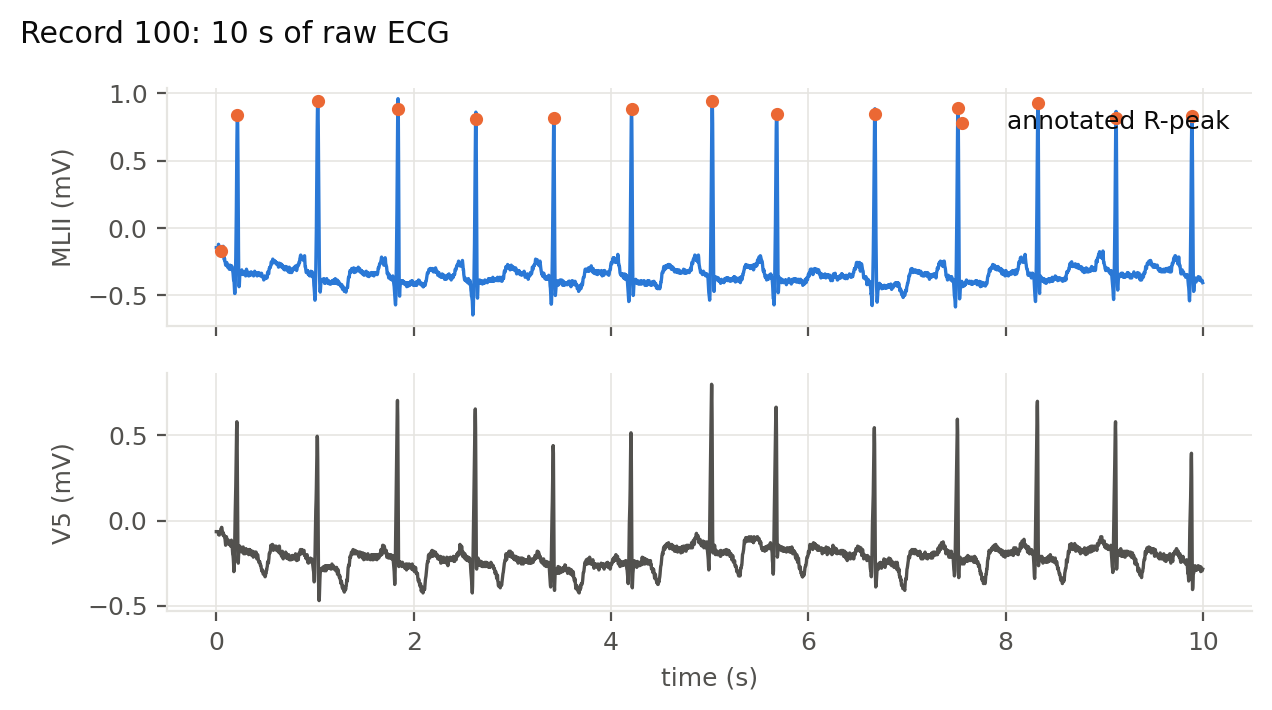
\includegraphics[width=\linewidth]{eda_raw_ecg.png}
  \caption{Ten seconds of raw ECG from record 100.}
  \label{fig:raw-ecg}
\end{figure}

\textbf{One beat per class.} Figure~\ref{fig:class-examples} shows a typical beat of each class, aligned on the R-peak. N and S beats are difficult to separate by shape; the main difference is timing, since the S beat arrives earlier than expected. The V beat has a wide QRS and no normal P wave. The F beat has an intermediate shape between N and V.

\begin{figure}[H]
  \centering
  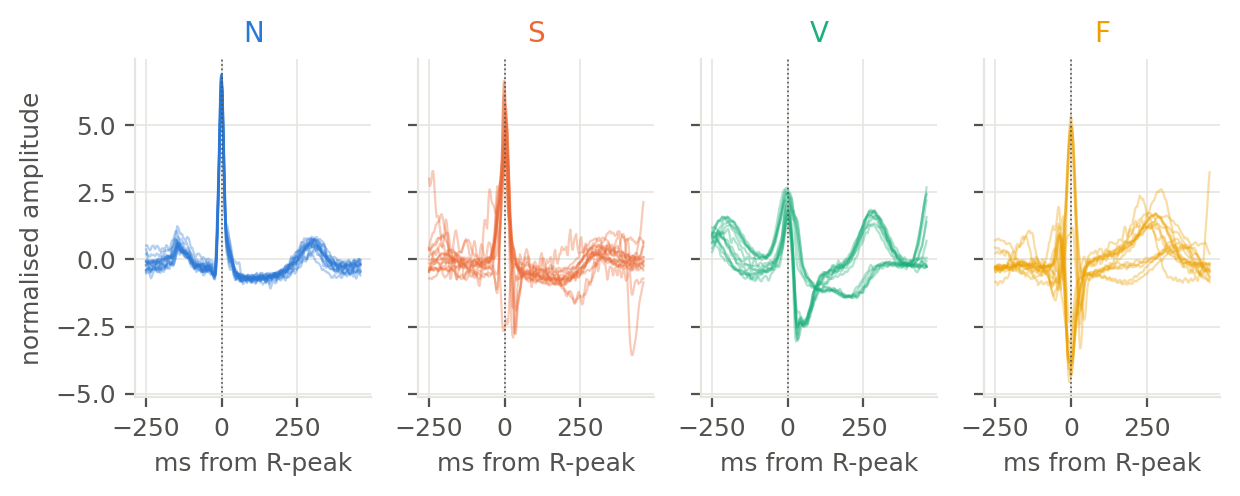
\includegraphics[width=\linewidth]{eda_class_examples.png}
  \caption{Example heartbeat of each class, 256-sample window centred on the R-peak.}
  \label{fig:class-examples}
\end{figure}

\textbf{Class distribution.} Figure~\ref{fig:class-dist} shows how uneven the classes are. Normal beats make up close to 90\,\% of the data, V beats are the largest minority, S beats are about 2--3\,\% and F beats well under 1\,\%. This imbalance motivates several decisions in Section~\ref{sec:data-preparation}.

\begin{figure}[H]
  \centering
  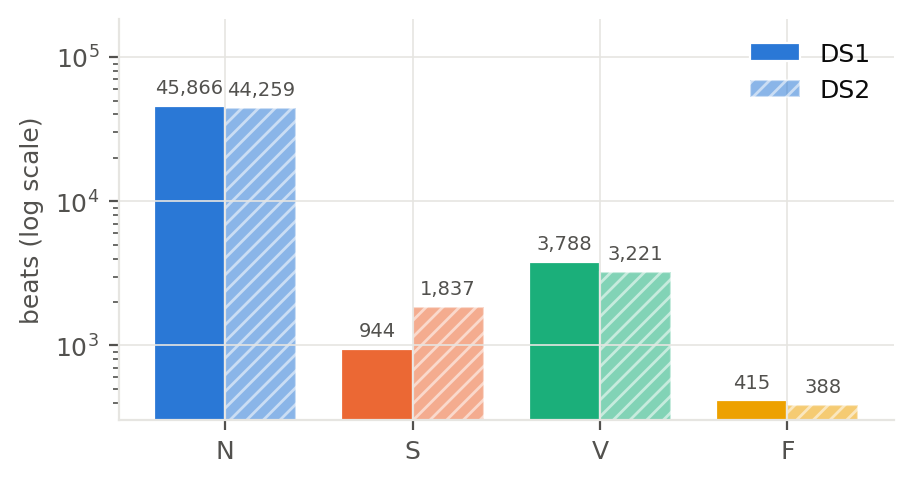
\includegraphics[width=\linewidth]{eda_class_distribution.png}
  \caption{Number of beats per class in DS1 and DS2 (logarithmic scale).}
  \label{fig:class-dist}
\end{figure}

\textbf{Beats per record.} Figure~\ref{fig:record-dist} shows the class composition of each record. The rare classes are not spread evenly: most S beats come from a few records such as 118, 207, 209 and 232, and most F beats from records 208 and 213. Performance on these classes therefore depends heavily on which records are in each split.

\begin{figure}[H]
  \centering
  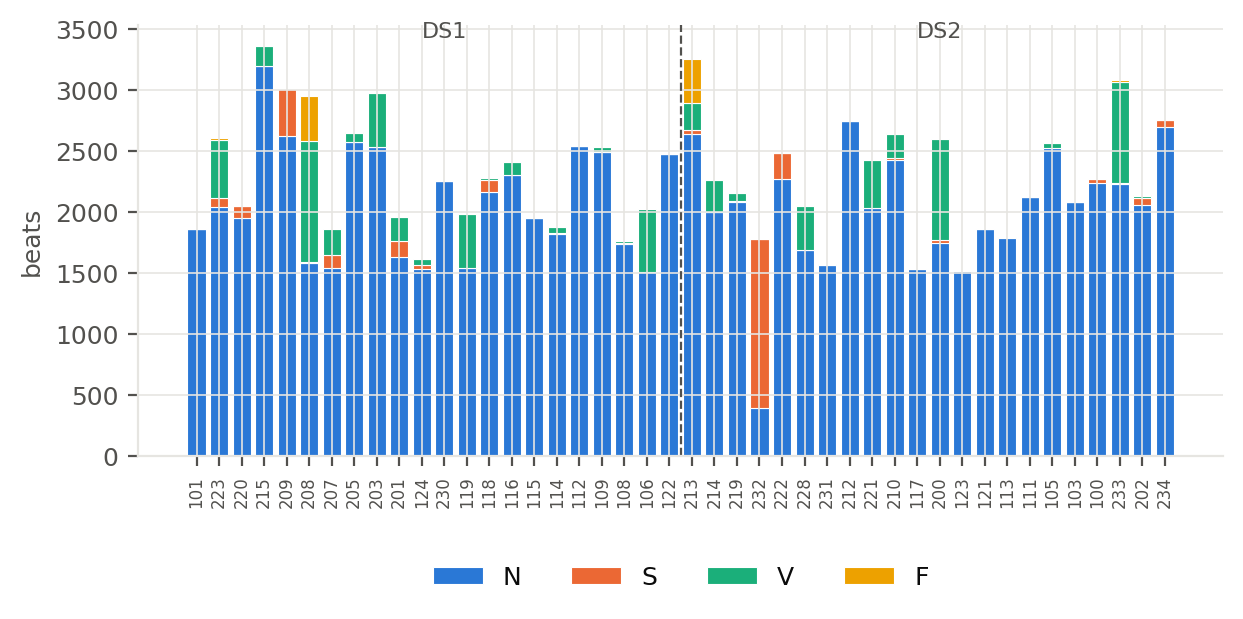
\includegraphics[width=\linewidth]{eda_record_distribution.png}
  \caption{Class composition of each record.}
  \label{fig:record-dist}
\end{figure}

\textbf{Signal amplitude.} Figure~\ref{fig:amplitude} shows the distribution of R-peak amplitude per record. Amplitudes vary by a factor of several between records because electrode placement and skin contact differ between subjects. Each beat is therefore normalised individually rather than with one global scale.

\begin{figure}[H]
  \centering
  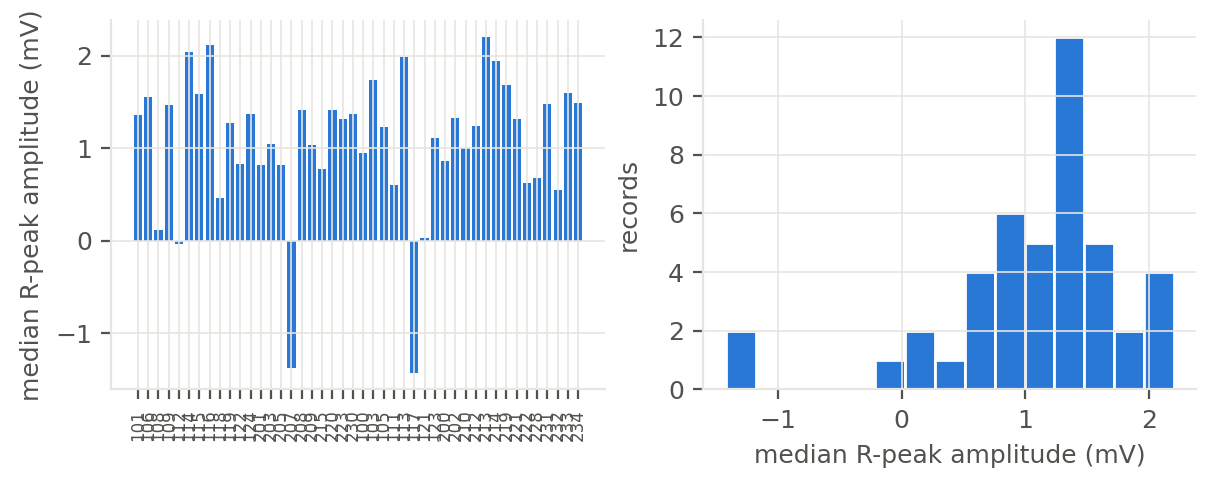
\includegraphics[width=\linewidth]{eda_amplitude.png}
  \caption{Distribution of R-peak amplitude across records.}
  \label{fig:amplitude}
\end{figure}

\textbf{Noisy ECG.} Figure~\ref{fig:noisy} shows segments from records 203 and 207, which are known to be noisy, together with the three noise types from the Noise Stress Test Database. Baseline wander is a slow drift, muscle artefact is high-frequency noise, and electrode motion produces abrupt transients that can resemble beats.

\begin{figure}[H]
  \centering
  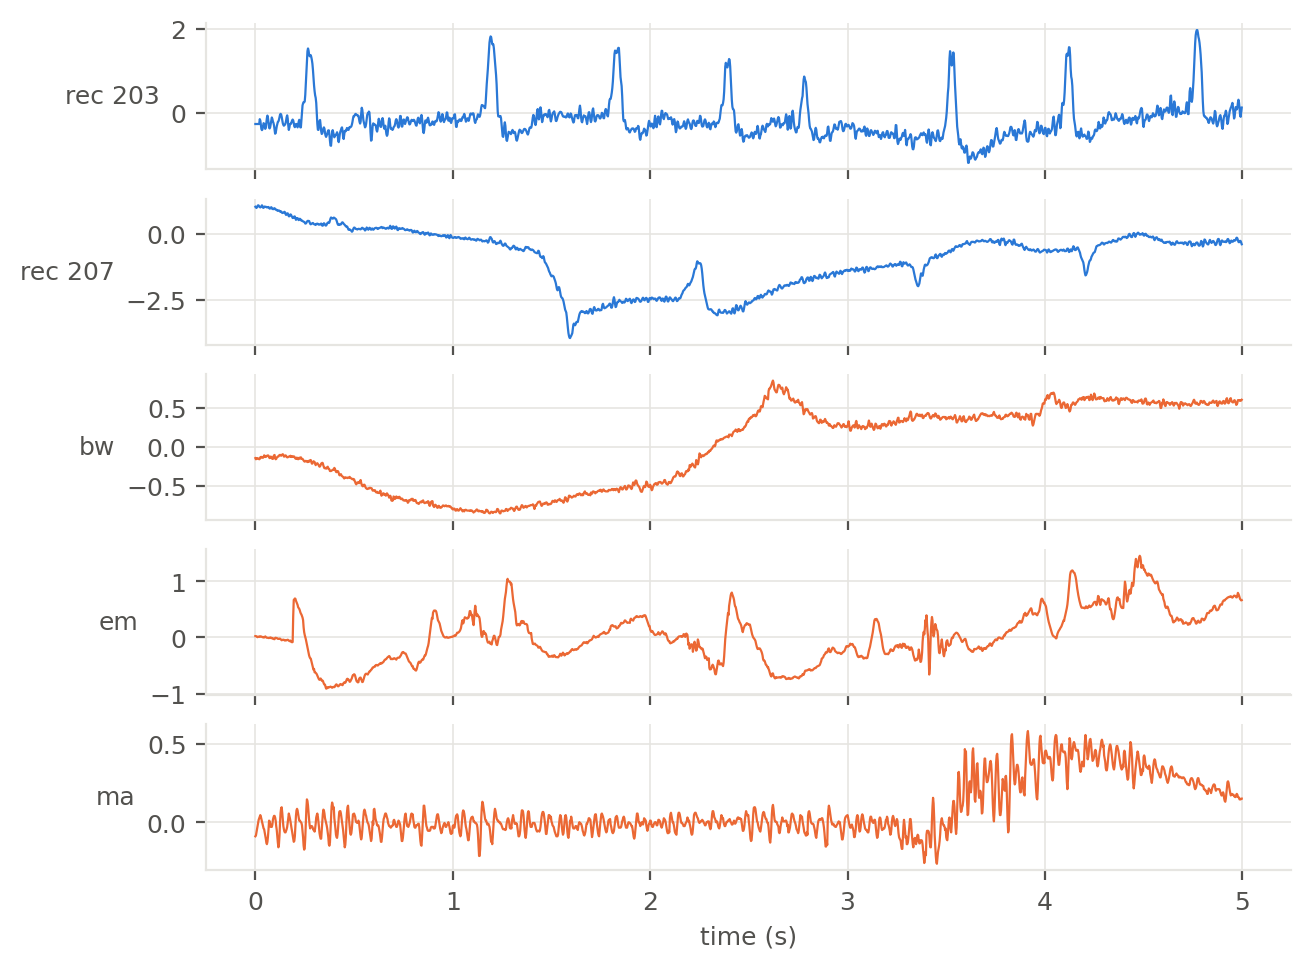
\includegraphics[width=\linewidth]{eda_noisy.png}
  \caption{Examples of noisy ECG and of the three noise types used in the robustness test.}
  \label{fig:noisy}
\end{figure}

\subsection{Data Quality}

\textbf{Missing data.} The recordings have no missing samples. Every record is complete at 360\,Hz.

\textbf{Extreme amplitudes.} A few records contain short bursts where the signal saturates at the limits of the 10\,mV range, usually during electrode movement. These segments are rare. Per-beat normalisation and clipping limit their effect on the input.

\textbf{Corrupted segments.} The annotators marked noisy stretches with the \texttt{\textasciitilde} symbol. Records 203, 207 and 208 contain the most of these. The beats inside these segments are kept, since a wearable will encounter the same kind of signal, but they are a likely source of label noise.

\textbf{Class imbalance.} Described above; it is the main data-quality issue.

\textbf{Differences between recordings.} Heart rate, beat shape, amplitude and noise level all vary from record to record. Some records show only normal rhythm, others show bundle branch block on every beat, and a few contain long runs of ventricular beats. Because of this variation, results on a small number of records can be misleading.

\textbf{Differences between channels.} MLII is the first channel in 46 of the 48 records, but in record 114 the two channels are stored in the opposite order. Selecting the lead by name rather than by column index avoids reading the wrong signal. Records 102 and 104 have no MLII; both are paced records and are already excluded.

\textbf{Possible noisy regions.} Baseline wander is present to some degree in almost every record. It is removed in preprocessing rather than detected and skipped.

\subsection{Leakage Analysis}

Data leakage occurs when information from the test set reaches the model during training, so the test score no longer measures generalisation.

A record is thirty minutes of ECG from one person. Its roughly 2\,000 beats share the same heart, electrodes and skin contact, so they are highly similar. If all beats were pooled, shuffled and split 80/20, nearly every test beat would have a near-duplicate in the training set. A model could then memorise each patient's waveform and exceed 99\,\% test accuracy without learning what distinguishes the classes. Studies using such splits report accuracies of this kind, which fall to 80--90\,\% when the same models are tested on unseen subjects. A wearable device only sees unseen subjects, so the shuffled score does not measure the quantity of interest.

Three measures prevent this. First, the data is split by record using the standard inter-patient partition: 22 records form the development set DS1 and 22 different records form the test set DS2, with no record in both. The partition has one known weakness: records 201 and 202 come from the same subject, and the standard split places 201 in DS1 and 202 in DS2. The partition is kept as published so that results remain comparable with the literature, and this is noted as a limitation. Second, the training/validation split inside DS1 is also by record, so model selection uses subjects the model was not trained on. Third, the split is enforced in code: the split-building function rejects a validation record that is not in DS1 and checks that no record is listed twice, and the evaluation script refuses to run on DS2 without an explicit \texttt{--final} flag. DS2 is used once per final model, after all design decisions are fixed.

The same rule applies to the noise experiment. Noise is added to DS2 only at evaluation time and the noisy signals are never used for training. Noise used as training augmentation is added to DS1 records only.

\section{Data Preparation}
\label{sec:data-preparation}

All steps in this section are implemented in \texttt{src/prepare\_data.py} and the \texttt{ecg.data} package. Every tunable number comes from \texttt{configs/preprocess.yaml}, so the whole pipeline can be rerun from the raw PhysioNet files with one command.

\subsection{Record Selection}
\label{sec:record-selection}

The split follows the inter-patient partition of de~Chazal et al.~\cite{dechazal2004}, as recommended by the assignment. The four paced records are excluded.

\begin{table}[H]
  \centering
  \caption{Record assignment. Training and validation together form DS1.}
  \label{tab:records}
  \rowcolors{2}{white}{rowtint}
  \begin{tabularx}{\linewidth}{l c Y}
        \rowcolor{primaryblue}
    \hd{Split} & \hd{Records} & \hd{Record numbers} \\
    Training (DS1 minus validation) & 17 & 101, 106, 108, 109, 112, 114, 115, 116, 119, 122, 207, 208, 209, 215, 220, 223, 230 \\
    Validation (subset of DS1)      & 5  & 118, 124, 201, 203, 205 \\
    Test (DS2)                      & 22 & 100, 103, 105, 111, 113, 117, 121, 123, 200, 202, 210, 212, 213, 214, 219, 221, 222, 228, 231, 232, 233, 234 \\
    \bottomrule
  \end{tabularx}

\end{table}

The validation records were chosen after inspecting the per-record class counts (Figure~\ref{fig:record-dist}). A first choice that placed record 208 in validation left only 20 fusion beats for training, because record 208 alone holds 372 of the 415 F beats in DS1. The final choice keeps records 208 and 209, which hold most of the F and S beats respectively, in training, and uses five records that together contain all four classes: 118 and 201 contribute S beats, 203 and 201 contribute V beats, and 124 and 205 contribute a few F beats. Validation therefore holds about 23\,\% of the DS1 beats but only 19 fusion beats, which is a limitation of the dataset rather than of the split; no assignment of DS1 records gives both training and validation a large F class. Validation is used for early stopping, hyperparameter choice and model selection. DS2 is not used until the final model is fixed.

\subsection{ECG Channel Selection}

A single lead, MLII, is used. It is present in every record used, it is the lead the annotators worked from, and it shows the QRS complex most clearly. A single lead also matches the wearable setting, where a patch or watch typically records one channel.

The lead is selected by its name in the record header rather than by position, because in record 114 MLII is stored as the second channel. If a record has no MLII the script raises an error rather than substituting another lead. This only affects records 102 and 104, which are excluded.

\subsection{Beat Extraction}

No beat detector is used. R-peak positions are taken from the expert annotation files, which is the standard approach for this database and keeps the project focused on classification.

Around each annotated R-peak a window of 90 samples before and 166 samples after the peak is extracted, giving a fixed input length of 256 samples, about 0.71 seconds at 360\,Hz. The window is asymmetric: 90 samples (250\,ms) before the peak covers the P wave, and 166 samples (460\,ms) after it covers the T wave at normal heart rates. A length of 256 is a power of two, which simplifies the memory layout on the MAX78002.

Beats whose window extends past the start or end of the recording are dropped, which affects at most one or two beats per record.

\subsection{Signal Preprocessing}

The operations are applied in this order:

\begin{center}
\texttt{Raw MLII signal}
$\rightarrow$ \texttt{baseline removal}
$\rightarrow$ \texttt{low-pass filter}
$\rightarrow$ \texttt{segmentation}
$\rightarrow$ \texttt{per-beat normalisation}
$\rightarrow$ \texttt{clipping}
$\rightarrow$ \texttt{model input (1$\times$256)}
\end{center}

\textbf{Baseline removal.} Two cascaded median filters with windows of 200\,ms and 600\,ms estimate the slow baseline, which is then subtracted from the signal. Breathing and body movement shift the baseline by more than the height of a QRS complex, so without this step identical beats at different points of the drift would look different to the model. A median filter removes the drift without distorting the QRS and is cheap enough to run on the microcontroller's CPU.

\textbf{Low-pass filter.} A zero-phase Butterworth filter with a 40\,Hz cut-off removes muscle noise and mains interference above the frequency range of the ECG itself. This step is optional in the configuration so that its effect can be measured in the noise experiment.

\textbf{Segmentation.} The filtered signal is cut into 256-sample windows as described above. Segmentation follows filtering so that the filters operate on a continuous signal and produce no edge effects inside a beat.

\textbf{Per-beat normalisation.} Each window is standardised to zero mean and unit standard deviation. Amplitude varies by a factor of several between subjects and electrode placements and carries no class information. Normalisation is applied per beat rather than per record because a wearable does not know the record statistics in advance.

\textbf{Clipping.} Values are clipped to the range $[-8, 8]$ standard deviations. This bounds the input, which 8-bit quantisation requires, and prevents a single electrode-motion spike from dominating the window. The limit was first set to 4, but inspection of the processed beats showed that R-peaks typically reach 5 to 7 standard deviations, so a limit of 4 flattened the peak on 74\,\% of beats and did so far more often for N and S beats than for V beats. A limit of 8 leaves all ordinary beats untouched. In the final step before the model the bounded range is mapped to the accelerator's input range of $[-1, 1)$.

\textbf{RR intervals.} Alongside each window, the time to the previous and next annotated beat is stored, together with the ratio of the previous interval to the mean of the ten intervals before it. These values are capped at 3 seconds, because unannotated episodes such as the 100-second ventricular flutter in record 207 would otherwise produce meaningless intervals. They are not part of the CNN input; the baseline uses them.

\subsection{Label Preparation}

The mapping from annotation symbol to class is a single dictionary in \texttt{src/ecg/constants.py}, reproduced here in full. Any symbol not listed is either an excluded beat or a non-beat annotation and is dropped with a count.

\begin{table}[H]
  \centering
  \caption{Complete label mapping.}
  \label{tab:label-mapping}
  \rowcolors{2}{white}{rowtint}
  \begin{tabularx}{\linewidth}{l Y c c}
        \rowcolor{primaryblue}
    \hd{Symbol} & \hd{PhysioNet description} & \hd{Class} & \hd{Index} \\
    \texttt{N} & Normal beat                          & N & 0 \\
    \texttt{L} & Left bundle branch block beat        & N & 0 \\
    \texttt{R} & Right bundle branch block beat       & N & 0 \\
    \texttt{e} & Atrial escape beat                   & N & 0 \\
    \texttt{j} & Nodal (junctional) escape beat       & N & 0 \\
    \texttt{A} & Atrial premature beat                & S & 1 \\
    \texttt{a} & Aberrated atrial premature beat      & S & 1 \\
    \texttt{J} & Nodal (junctional) premature beat    & S & 1 \\
    \texttt{S} & Supraventricular premature beat      & S & 1 \\
    \texttt{V} & Premature ventricular contraction    & V & 2 \\
    \texttt{E} & Ventricular escape beat              & V & 2 \\
    \texttt{F} & Fusion of ventricular and normal beat & F & 3 \\
    \midrule
    \texttt{/}, \texttt{f}, \texttt{Q} & Paced, fusion of paced and normal, unclassifiable & excluded & -- \\
    others & Rhythm, noise and signal-quality annotations & not a beat & -- \\
    \bottomrule
  \end{tabularx}

\end{table}

\subsection{Class Imbalance}

In the training set roughly 89.6\,\% of beats are normal, 1.7\,\% are S, 7.6\,\% are V and 1.0\,\% are F, so the ratio between the most and least common class is about 90 to one. With plain cross-entropy a network converges towards predicting N almost always, because that minimises the loss.

Two measures are combined. First, a \textbf{class-weighted cross-entropy loss}, with each class weighted by the inverse square root of its frequency; the square root moderates the weights so that rare classes are emphasised without destabilising training. Second, \textbf{oversampling of S and F} in the training sampler, so that each batch contains more minority beats than their natural share.

Undersampling normal beats would discard most of the data. Focal loss is kept as a configurable alternative for model selection, and no balancing is included as a negative control. The final choice is made on validation macro-F1 and S/F recall, not on the test set.

\subsection{Data Augmentation}

Augmentation is applied on the fly to training beats only. Validation and test beats are never augmented, so the validation score remains an unbiased estimate. Each transformation is a small random change that preserves the class:

\begin{itemize}[nosep]
  \item \textbf{Amplitude scaling} by a random factor between 0.8 and 1.2, since amplitude carries no class information.
  \item \textbf{Time shift} of up to $\pm 5$ samples, so the model tolerates small errors in R-peak alignment.
  \item \textbf{Baseline wander}, a low-frequency sinusoid added to the window, to prepare the model for imperfect baseline removal.
  \item \textbf{Gaussian noise} with a standard deviation of about 0.02 after normalisation.
  \item \textbf{Real ECG noise} from the Noise Stress Test Database at a signal-to-noise ratio of 6\,dB or better, as an optional setting. One model is trained with and one without it to measure the effect in the noise experiment.
\end{itemize}

Beats are not stretched or compressed in time. QRS width is one of the main features separating V from N beats, so changing it would corrupt the labels.

\subsection{Final Dataset}

\begin{table}[H]
  \centering
  \caption{Beat counts per split, produced by \texttt{prepare\_data.py} and stored in \texttt{results/split\_stats.csv}.}
  \label{tab:final-dataset}
  \rowcolors{2}{white}{rowtint}
  \begin{tabularx}{\linewidth}{l c R R R R R}
        \rowcolor{primaryblue}
    \hd{Split} & \hd{Records} & \hd{N} & \hd{S} & \hd{V} & \hd{F} & \hd{Total} \\
    Train & 17 & 35\,414 & 684 & 3\,012 & 395 & 39\,505 \\
    Validation & 5 & 10\,434 & 260 & 776 & 19 & 11\,489 \\
    Test (DS2) & 22 & 44\,240 & 1\,837 & 3\,220 & 388 & 49\,685 \\
    \bottomrule
  \end{tabularx}

\end{table}

\subsection{Reproducibility}

\begin{table}[H]
  \centering
  \caption{Settings needed to reproduce the preprocessing. All are stored in \texttt{configs/preprocess.yaml}.}
  \label{tab:reproducibility}
  \rowcolors{2}{white}{rowtint}
  \begin{tabularx}{\linewidth}{l Y}
        \rowcolor{primaryblue}
    \hd{Item} & \hd{Value} \\
    Python             & 3.10 \\
    Key packages       & wfdb 4.3.1, NumPy 2.2.6, SciPy 1.15.3, scikit-learn 1.7.2; exact versions in \texttt{requirements.txt} \\
    Random seed        & 42, applied to Python, NumPy and PyTorch \\
    Sampling frequency & 360\,Hz, no resampling \\
    Lead               & MLII, selected by name \\
    Window             & 90 samples before the R-peak, 166 after; input size $1 \times 256$ \\
    Baseline removal   & Cascaded median filters, 200\,ms and 600\,ms \\
    Low-pass filter    & Butterworth, 40\,Hz cut-off, zero-phase \\
    Normalisation      & Per-beat z-score, clipped to $[-8, 8]$ \\
    Data source        & PhysioNet \texttt{mitdb} 1.0.0 and \texttt{nstdb} 1.0.0, downloaded with the \texttt{wfdb} package \\
    \bottomrule
  \end{tabularx}

\end{table}

Running the following command from a clean checkout, after downloading the data, regenerates every array and every number in this section:
\begin{center}
\texttt{python src/prepare\_data.py --config configs/preprocess.yaml}
\end{center}


% ===== Submission 2: CRISP-DM stages 4-6 =====
\section{Modeling}

\subsection{Baseline}
% At least one simple baseline and its performance.

\subsection{Proposed Edge Model}
\begin{table}[H]
  \centering
  \begin{tabular}{@{}lllll@{}}
    \toprule
    Layer & Input & Operation & Output & Parameters \\
    \midrule
     &  &  &  &  \\
    \bottomrule
  \end{tabular}
  \caption{Edge model architecture.}
  \label{tab:architecture}
\end{table}
% Explain why this architecture is appropriate for Edge-AI.

\subsection{Training Configuration}
% optimizer, learning rate, batch size, epochs, loss function, early stopping,
% class weighting, augmentation, random seed.

\subsection{Model Selection}
% Models tried, hyperparameters varied, validation metric used, why the final architecture was selected.

\subsection{Quantization}
% FP32 vs INT8. If QAT is used: why it is needed, how it was performed, whether performance changed.

\section{Evaluation}

\subsection{Clean Test Results}
\begin{table}[H]
  \centering
  \begin{tabular}{@{}lrrr@{}}
    \toprule
    Metric & Baseline & FP32 Edge Model & Quantized Model \\
    \midrule
    Accuracy         &  &  &  \\
    Macro F1         &  &  &  \\
    Model parameters &  &  &  \\
    \bottomrule
  \end{tabular}
  \caption{Clean DS2 test results.}
  \label{tab:clean-results}
\end{table}

\subsection{Per-Class Performance}
\begin{table}[H]
  \centering
  \begin{tabular}{@{}lrrr@{}}
    \toprule
    Class & Precision & Sensitivity/Recall & F1 \\
    \midrule
    N &  &  &  \\
    S &  &  &  \\
    V &  &  &  \\
    F &  &  &  \\
    \bottomrule
  \end{tabular}
  \caption{Per-class performance of the final model on DS2.}
  \label{tab:per-class}
\end{table}
% Confusion matrix figure; discuss which classes are difficult and why.

\subsection{Quantization Analysis}
\begin{itemize}
  \item FP32 Macro F1: \rule{2cm}{0.4pt}
  \item INT8 Macro F1: \rule{2cm}{0.4pt}
  \item Difference: \rule{2cm}{0.4pt}
\end{itemize}

\subsection{Noise Robustness}
\begin{table}[H]
  \centering
  \begin{tabular}{@{}lrr@{}}
    \toprule
    Condition & Accuracy & Macro F1 \\
    \midrule
    Clean &  &  \\
    12 dB &  &  \\
    6 dB  &  &  \\
    0 dB  &  &  \\
    \bottomrule
  \end{tabular}
  \caption{Performance under increasing ECG noise.}
  \label{tab:noise}
\end{table}
% Plot performance vs noise level. Discuss: most affected classes, gradual degradation,
% whether preprocessing helps, whether robustness could be improved.

\subsection{Error Analysis}
% Representative errors with ECG waveforms: N->S, S->N, V misclassified, errors under strong noise.

\subsection{Success Criteria Review}
% For each criterion from Section 1.4: Achieved / Partially achieved / Not achieved, with justification.

\section{Deployment}

\subsection{MAX78002 Compatibility}
% Why the architecture runs on the CNN accelerator, layer types, input/output dimensions, parameter count.

\subsection{MAX78002 Toolchain}
% ai8x-training and ai8x-synthesis: preparation, quantization, synthesis, C code generation.

\subsection{Deployment Evidence}
\begin{table}[H]
  \centering
  \begin{tabular}{@{}ll@{}}
    \toprule
    Requirement & Result \\
    \midrule
    Model accepted by MAX78002 toolchain & PASS / FAIL \\
    Quantization completed               & PASS / FAIL \\
    Synthesis completed                  & PASS / FAIL \\
    C/device files generated             & PASS / FAIL \\
    Weight memory requirement            &  \\
    Data memory requirement              &  \\
    \bottomrule
  \end{tabular}
  \caption{Synthesis evidence.}
  \label{tab:deployment-evidence}
\end{table}

\subsection{Hardware Limitations}
% No measured latency, power, energy, real accuracy or real-time claims.
% Clearly distinguish software verified versus hardware verified.

\subsection{Proposed Hardware Validation}
% Loading the model, identical inputs, Python vs hardware output comparison,
% intermediate/final consistency, inference time, energy consumption.

\section{Final Discussion}
% What did you learn from the data? Biggest source of error? Was the highest-accuracy model
% also the best Edge-AI model? Performance lost after quantization? Sensitivity to noise?
% Compromises due to hardware constraints? What would you change with more time?

\section{Limitations}
% limited dataset size, class imbalance, differences between patients, use of historical
% ECG datasets, absence of prospective clinical testing, lack of hardware testing,
% possible domain shift to wearable ECG devices.


% ============================= References ============================
\newpage
\printbibliography
\addcontentsline{toc}{section}{References}

\end{document}
